\sloppy
\documentclass[14pt,a4paper,oneside]{extarticle}	% Размер основного шрифта и формата листа
\usepackage{xltxtra}						% Используется для вывода логотипа XeLaTeX
\usepackage{xunicode}						% Кодировка документа
\usepackage{polyglossia}					% Загружает пакет многоязыковой верстки
\newfontfamily\russianfont{Book Antiqua}
%\setmainfont{Liberation Serif}						% Основной шрифт текста
\setmainfont{Book Antiqua}
\setdefaultlanguage{russian}				% Основной язык текста
\setotherlanguage{english}					% Дополнительный язык текста
\linespread{1}							% Межстрочный интервал выбран полуторным
\usepackage[left=2.5cm,
right=1.5cm,vmargin=2.5cm]{geometry} % Отступы по краям листа
\bibliographystyle{ugost2008}

\usepackage{xcolor}
\usepackage{hyperref}
% Цвета для гиперссылок
\definecolor{linkcolor}{HTML}{359B08} % цвет ссылок
\definecolor{urlcolor}{HTML}{799B03} % цвет гиперссылок
\hypersetup{pdfstartview=FitH,  linkcolor=linkcolor,urlcolor=urlcolor, colorlinks=true}

%---------------------------%
%---- Пакеты расширений ----%
%---------------------------%
\usepackage{xcolor}
\usepackage{hyperref}
% Цвета для гиперссылок
\definecolor{linkcolor}{HTML}{359B08} % цвет ссылок
\definecolor{urlcolor}{HTML}{799B03} % цвет гиперссылок
\hypersetup{pdfstartview=FitH,  linkcolor=linkcolor,urlcolor=urlcolor, colorlinks=true}


\usepackage{verbatim,indentfirst}
\usepackage{cite,enumerate,float}
\usepackage{amsmath,amssymb,amsthm,amsfonts}

%---------------------------%
%--- Вставка иллюстраций ---%
%---------------------------%
\usepackage{graphicx}
\usepackage{subfigure}
%\graphicspath{{Images/}}
\usepackage{fontspec}

\begin{document}
%	\pagestyle{empty} %  выключаенм нумерацию

	%\setcounter{page}{3}% Нумерация начинается с третьей страницы
	%\renewcommand{\contentsname}{\center{Содержание}}
	%\tableofcontents
	
\begin{center}
		%\addcontentsline{toc}{section}{Опыт 14. Вязкое трение}
		\subsection*{Сухое и жидкое трение}
\end{center}
	
	\begin{figure}[H] 	% Окружение для вставки иллюстрации
		\centering 	
		% Выравнивание по центру
		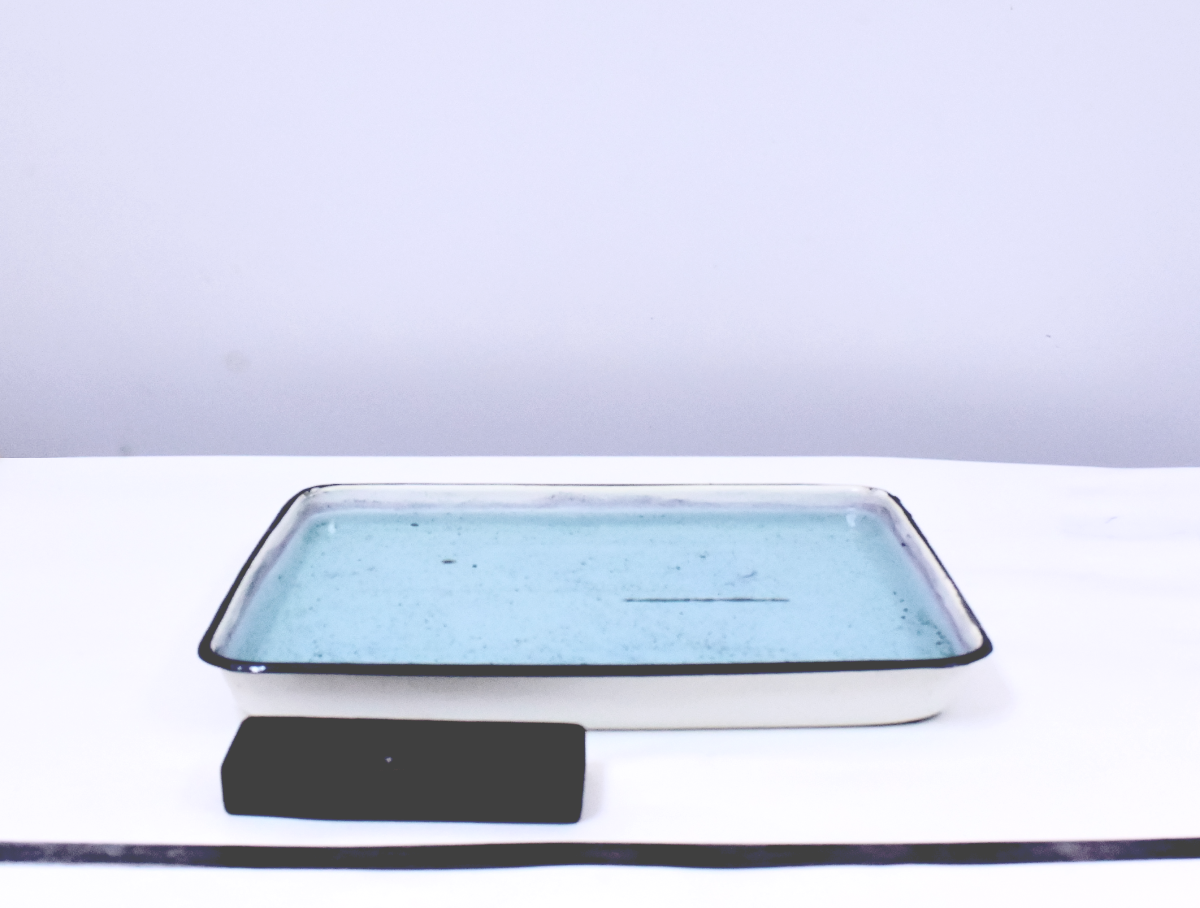
\includegraphics[width=0.9\linewidth]{friction-1.png}
		\caption{Демонстрация отсутствия у ньютоновской жидкости такого свойства как трение покоя (начальное напряжение сдвига)}
		\label{friction-1}
	\end{figure}
	
	\subsection*{\underline{Оборудование:}}
	
	\begin{enumerate} 
		\item Деревянный брусок 
		\item Упругая пластина (металлическая линейка)
		\item Кювета с водой
		
	\end{enumerate}

	\newpage	
	\subsection*{\underline{Основные определения:}}
	
	Силы, возникающие при движении тел в газе или жидкости 
	и зависящие от скорости их относительного движения, называются 
	силами вязкого (жидкого) трения или силами сопротивления среды. 
	Силы трения всегда направлены в сторону, противоположную скорости относительного 
	движения.
	Кроме того, они также направлены по касательной к соприкасающимся поверхностям.
		
	В общем виде закон, связывающий силу жидкого трения \textbf{\textit{f}} со 
	скоростью \textbf{v} движения тел относительно жидкости или газа, очень 
	сложен и для больших скоростей не может быть передан простой 
	формулой. 
	Для движения тел с малыми скоростями можно считать, что сила жидкого трения \textit{\textbf{f}}, действующая на движущиеся в жидких средах тела, пропорциональна скорости относительного движения этих тел \textbf{v}.
	Учитывая, что направления скорости и силы жидкого трения противоположны, можно написать: 
$$
	\textit{\textbf{f}} \sim - \eta \textbf{v}S,
$$
	а для больших скоростей 
$$
	f \sim v^2.
$$
	
	Коэффициент пропорциональности $ \eta $ называется коэффициентом жидкого трения или коэффициентом сопротивления среды. 
	Его значение зависит от размеров и формы движущегося тела, а также от свойств жидкости или газа.
	Здесь величина \textit{S} обозначает площадь слоя (поверхности тела), по которому происходит сдвиг.
	
	Ньютоновская жидкость — такая вязкая жидкость, которая при своем течении подчиняется закону вязкого трения Ньютона. 
	Свойствами ньютоновской жидкости обладают большинство жидкостей (вода, смазочное масло и др.) и все газы. 
	Течение ньютоновских жидкостей изучается в гидроаэромеханике. 
	
	Жидкости, для которых закон вязкого трения Ньютона выполняется,	называются неньютоновскими.
	К ним относится ряд суспензий и растворов полимеров. 
	Такие течения изучает реология.

	\newpage	
	\subsection*{\underline{Краткое описание:}}
	
	На демонстрационном столе располагается плоская ванна с водой.
	Рядом с ванной находится прямоугольный деревянный брусок с гладкой поверхностью.
	На брусок при помощи гибкой металлической пластинки оказывается давление так, что один из концов пластинки касается края бруска(рис.\ref{friction-2},\textit{а}).
	Опыт показывает, что при небольшой деформации самой линейки тело остается в покое, 
	а если постепенно увеличивать силу давления на брусок, то тело способно придти в движение в сторону приложения силы.
	Однако деформация линейки в таком случае окажется значительной.
		
	Важно отметить, что вес бруска будет равен максимальной силе трения покоя.
	Если поставить на брусок груз, вес которого равен весу бруска, то вес движимого тела возрастет вдвое.
	При этом для приведения в движение системы с увеличенной массой необходимо приложить большую силу (изгиб линейки при этом увеличится).
	Следовательно, коэффициент трения бруска о поверхность стола останется постоянным.
	
		\begin{figure}[H] 
		\centering 	
		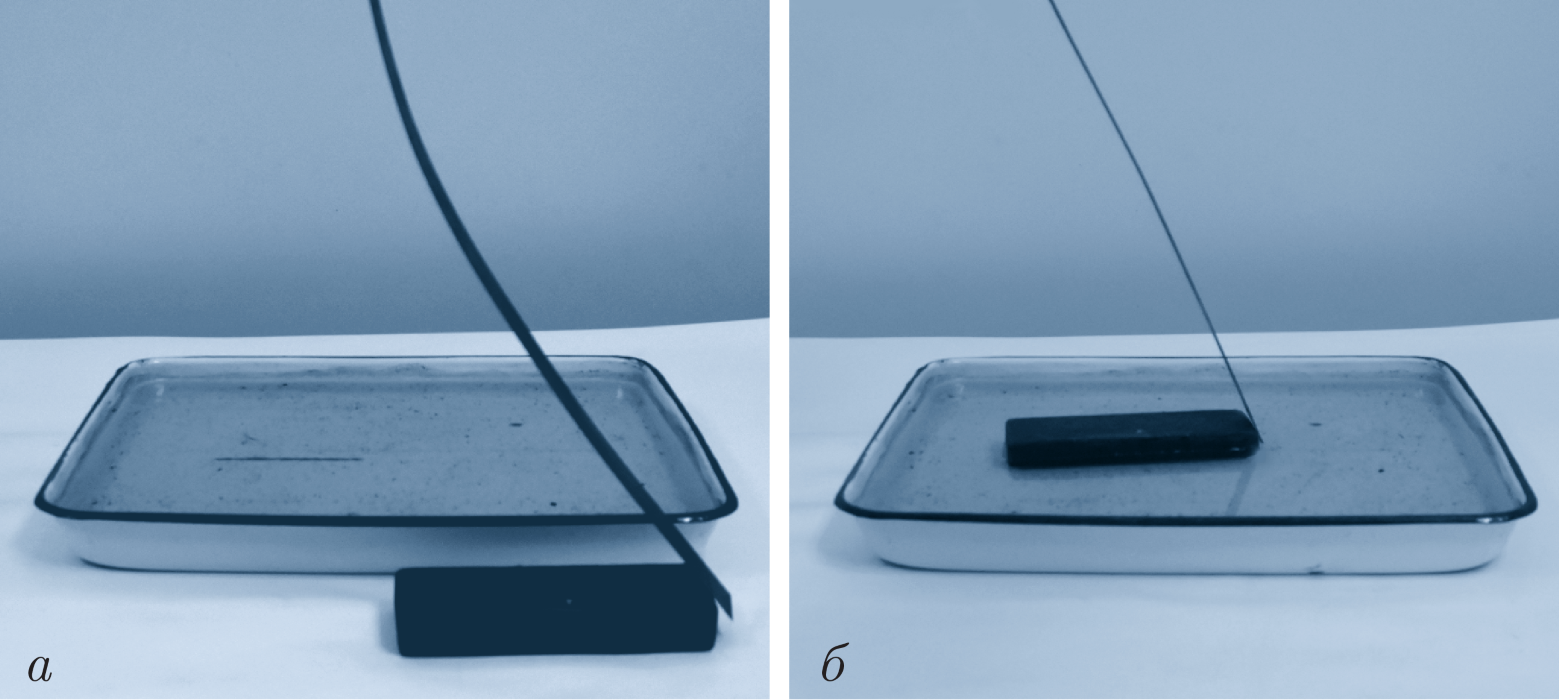
\includegraphics[width=0.75\linewidth]{friction-2.png}
		\caption{\textit{а} — чтобы привести брусок в движение по столу необходимо приложить заметное усилие, которое можно оценить по величине изгиба упругой пластинки; \textit{б} — при погружении бруска в воду его движение возникает при бесконечно малом усилии (пластинка не изгибается) }
		\label{friction-2}
	\end{figure}

	Для демонстрации жидкого трения брусок помещается на поверхность воды.
	В ходе опыта можно заметить, что брусок начинает двигаться по воде под влиянием едва действующей на него линейки.
	В этом случае коэффициент трения оказывается настолько малым, что линейка, 
	которой действуют на брусок, практически не деформируется (рис.\ref{friction-2},\textit{б}).
	Кроме того, можно показать, что брусок начнет двигаться по воде даже в том случае, 
	если слегка на него подуть.
	


	\newpage	
\subsection*{\underline{Теория:}}

Опыт позволяет показать, что для перемещения деревянного бруска вдоль свободной поверхности слоя жидкости с постоянной скоростью \textit{v} необходимо действовать на него с вполне определенной силой \textit{\textbf{F}}.
Причем в случае равномерного перемещения действие внешней силы \textit{\textbf{F}} уравновешивается равной ей по величине противоположно направленной силой трения \textit{\textbf{f}}.

	\begin{figure}[H] 
	\centering 	
	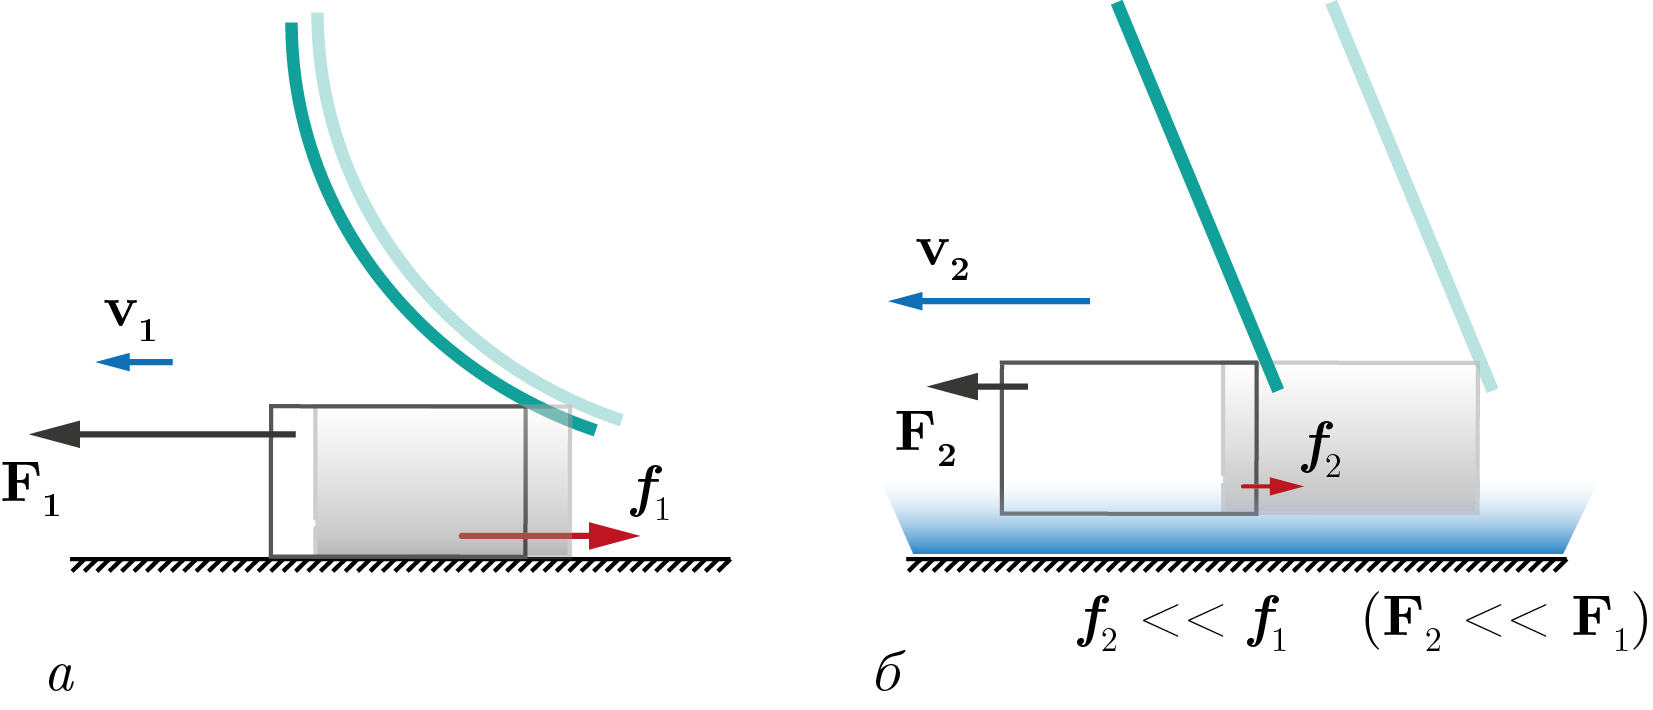
\includegraphics[width=0.9\linewidth]{friction-3.png}
	\caption{\textit{а} — схематичное изображение тела на горизонтальной поверхности и действующие на него силы; \textit{б} — распределение сил, действующих на груз, скатывающийся вдоль наклонной плоскости}
	\label{friction-3}
\end{figure}

Самое важное в характере сил вязкого трения то, что брусок начинает движение под действием очень малой силы ($ \textbf{F}_2 << \textbf{F}_1 $).
Таким образом, можно утверждать, что для жидкости не существует трения покоя. 
Это отличает вязкое трение от сухого.
	
\end{document}